\documentclass[11pt]{article}
\usepackage{fullpage}

\usepackage[hidelinks]{hyperref}

\usepackage{graphicx}

\usepackage{multicol,multirow}
\usepackage{caption}
\usepackage{amsmath, amssymb, amsthm}
\usepackage{setspace}
\usepackage{pdfpages}

\usepackage{subcaption}

\usepackage[sortcites,style=nature,sorting=none,backend=biber]{biblatex}
\addbibresource{ref.bib}

\theoremstyle{definition}
\newtheorem{theo}{\textbf{Theorem}}
\newtheorem{prp}{\large{Proposition}}
\newtheorem{defff}{\large{Defenition}}
\newtheorem{lem}{\large{Lemma}}
\renewcommand{\baselinestretch}{1.25}

\title{Population Dynamics of Bactria inside Humans}

\date{}
\setstretch{1.45}


\begin{document}
	\graphicspath{{../figs/}}
	
		\vspace*{\fill}
	\begin{figure}[htp]
		\centering 
\includegraphics[width = 3.5cm]{ut.png}
	\end{figure}
	\begin{center}
		\large
		College of Science
		\\
		School of Mathematics, Statistics and Computer Science
		\\
		{\LARGE Dynamics of Bacteria and antibiotic} \\
		\vspace{1cm}
		Professor: Dr. Arta Jamshidi
		\\
		\vspace{1cm}
		Students:\\
		Pooria Assarehha\\
		Mohammad Hossein Naderi\\
		Mani Moradi\\
		% EDIT HERE:
		\vspace{1cm}
		Numerical Analysis Project
		\\		
		Summer 2025
		\vspace{2cm}
	\end{center}
	\thispagestyle{empty}
	\vspace*{\fill}
	
	\newpage
	\setcounter{page}{2}
	
	\begin{center}
		\LARGE{\textbf{Abstract}}
		
		\vspace{1cm}
		
		
	\end{center}
	
	\begin{flushleft}
		\Large 
		Understanding the dynamics of interactions between antibiotic-resistant 	bacteria, the immune
		response, and the presence of antibiotics is crucial for developing effective strategies to combat
		antibiotic resistance. In this work, we introduce an innovative mathematical model that delves
		into the complex dynamics between bacteria that are resistant to antibiotics, the immune
		system, and the administration of antibiotic treatment. Through qualitative analysis, four
		distinct stable equilibria have been identified, each representing distinct biological scenarios,
		providing valuable insights for combating antibiotic resistance.
		
	\end{flushleft}
	
	\newpage	
	
	\tableofcontents
	
	\newpage
	
	\section{Introduction} 
	Antibiotic resistance constitutes a critical global health threat, with World Health Organization projections indicating potential annual mortality in the millions by 2050 if current trends persist. This project develops a mathematical framework for modeling bacterial population dynamics within the human body, specifically examining the tripartite interaction between pathogenic bacteria, host immune response, and antibiotic interventions. 
	
	\subsection{Problem Context}
	Traditional models of bacterial dynamics exhibit a significant limitation: they typically isolate either antibiotic effects \textit{or} immune response mechanisms. This fragmentation neglects the synergistic reality where:
	\begin{enumerate}
		\item \textbf{Antibiotic-resistant bacteria (ARB)} employ survival mechanisms including target-site modification and plasmid-mediated resistance gene transfer
		\item \textbf{Non-resistant bacteria} compete for resources while responding differently to selective pressures
		\item \textbf{Immune effectors} dynamically interact with both bacterial subpopulations
		\item \textbf{Antibiotics} simultaneously impose selective pressure while modulating immune activity
	\end{enumerate}
	The clinical urgency is underscored by resistance drivers such as antibiotic overuse (e.g., inappropriate viral infection treatment), premature therapy discontinuation, and incorrect dosing—all contributing to evolutionary selection favoring resistant strains.
	
	\subsection{Modeling Imperatives}
	Treatment complexity escalates dramatically with resistance emergence due to:
	\begin{itemize}
		\item Diminished therapeutic options with higher toxicity profiles
		\item Immune function degradation during severe infections
		\item \textbf{Selective pressure} phenomena where indiscriminate antibiotic use eliminates susceptible bacteria while creating ecological niches for ARB expansion
	\end{itemize}
	Epidemiological evidence suggests that modest reductions (e.g., 10\%) in unnecessary antibiotic usage could significantly curb resistance propagation. However, predicting intervention outcomes requires sophisticated modeling accounting for:
	\begin{equation*}
		\underbrace{\text{Bacterial growth kinetics}}_\text{Competition} + \underbrace{\text{Resistance transmission}}_\text{Horizontal transfer} + \underbrace{\text{Immune recruitment}}_\text{Nonlinear dynamics}
	\end{equation*}
	
	\subsection{Proposed Framework}
	Our novel dynamical system addresses existing gaps by concurrently integrating:
	\begin{itemize}
		\item Dual bacterial subpopulations (resistant vs. susceptible)
		\item Adaptive immune response dynamics
		\item Pharmacokinetic/pharmacodynamic antibiotic profiles
	\end{itemize}
	This tripartite model enables quantitative investigation of:
	\begin{itemize}
		\item Equilibrium conditions governing pathogen clearance
		\item Resistance dominance thresholds
		\item Chronic infection persistence criteria
	\end{itemize}
	Through numerical analysis and computational implementation, we examine critical scenarios including:
	\begin{itemize}
		\item Optimal dosing windows minimizing resistance selection
		\item Immune augmentation strategies complementing antibiotics
		\item Failure modes under subtherapeutic drug concentrations
	\end{itemize}
	
	\subsection{Structural Overview}
	This paper proceeds as follows: Section 2 formalizes key biological mechanisms; Section 3 develops the governing equations; Section 4 analyzes equilibrium states; Section 5 presents numerical simulations; and Section 6 details the open-source implementation. Our integrated approach provides a critical tool for simulating combination therapies and optimizing antimicrobial stewardship policies.

	
	
	\newpage
	\section{Dynamic Model} In our study, we introduce a detailed mathematical model designed to capture the behavior of bacterial populations,
including both non-resistant and resistant strains, along with their interactions with immune cells responsible for host defense, all
within the context of antibiotic presence. Our model is built upon several key assumptions, including considerations for bacterial reproduction and death rates, the transfer of antibiotic resistance genes between bacterial strains, the impact of the antibiotic itself,
and the response of the immune system. This complex interplay is described by a system of differential equations, which outlines
the dynamic relationships between these variables and processes:

\begin{equation}
	\begin{cases}
		\dot{A}(t)  =  \Lambda - \mu A, \\
		\dot{S}(t)  =  \eta_s\left(1 - \frac{S+R}{K}\right)S - \bar{\alpha}AS - \beta\frac{SR}{N} - \Gamma SP, \\
		\dot{R}(t)  =  \eta_r\left(1 - \frac{S+R}{K}\right)R + \beta\frac{SR}{N} - \Gamma RP, \\
		\dot{P}(t)  =  \Phi(N)P\left(1 - \frac{P}{P_{\max}}\right) - \Psi(N)P, \\
	\end{cases}
\end{equation}
where $S$ represents the population of Non-Antibiotic Resistant Bacteria (NARB), $R$ stands for the population of Antibiotic Resistant
Bacteria (ARB), $P$ denotes the population of immune cells and $A$ indicates the concentration of antibiotic.

\begin{figure}
	\centering
	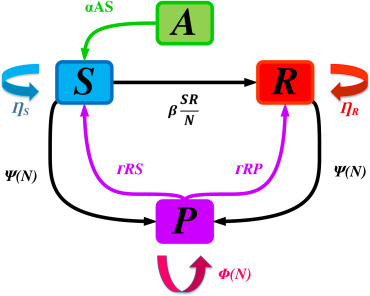
\includegraphics[width=0.6\textwidth]{1-s2.0-S1007570424005975-gr1.jpg}
	\caption{Schematic Diagram}
\end{figure}

In biological systems, the proliferation of ARB is frequently reported to exhibit a slower rate compared to NARB, owing to
a multitude of underlying reasons. These factors may include the metabolic costs associated with maintaining resistance
mechanisms, alterations in cellular physiology resulting from genetic mutations, and potential trade-offs between resistance and
other cellular functions. This phenomenon is significant as it impacts the overall dynamics of bacterial populations within ecosystems
and during infection processes. In our model, we incorporate a logistic growth terms characterized by growth rates $\eta_s$ for NARB and
$\eta_r$ for ARB, with $\eta_s > \eta_r$ , alongside a shared carrying capacity $K$.

Here, we look at how a resistance plasmid helps antibiotic-resistant genes move from bacteria types that are already resistant
to those that are not (susceptible strains). This plasmid serves as a means for the transfer of antibiotic resistance determinants
between bacteria. Biologically, this transfer is analogously perceived as analogous to the contagion dynamics observed in disease
transmission: a resistant bacterium (acting as the donor) encounters a non-resistant bacterium (the recipient), and the likelihood is
that both bacteria acquire resistance traits subsequent to the interaction. In this case, we employ the term: $\beta\frac{SR}{N}$.

The terms $\Gamma SP$ and $\Gamma RP$ describe the elimination of (NARB) and (ARB) by the immune cells. The final equation is
supported by the observed relationship between the potency of the immune response and the concentration of bacteria. Specifically,
a minor infection initiates an immune reaction, while a major infection dampens the immune response, either through the death of
immune cells or by impeding the proliferation of immune cells. $P_max$ is the maximum number of immune cells and the functions
$\Phi(N)$ and $\Psi(N)$ are supposed to be positive and belonging to $\mathrm{C}^1(\mathbb{R}_+)$.

Ultimately, the antibiotic is administered at a rate denoted by $\lambda$ and absorbed at a rate represented by $\mu$.

This model system has 9 parameters in all, which makes mathematical analysis complicated. We are going to review the
following transformation of variables:
\[ 
\begin{array}{ccccc}
	a = \frac{A}{\Lambda/\mu},\hspace{2mm} s = \frac{S}{K},\hspace{2mm} r = \frac{R}{K},\hspace{2mm} p = \frac{P}{P_{\max}},
	\hspace{2mm}
	\alpha = \frac{\bar{\alpha}A}{\mu},\hspace{2mm} \\ \gamma = \Gamma P_{\max},
	\hspace{2mm} n = s + r
\end{array}
\]

With the scaling, system (1) takes the form

\begin{equation}
	\begin{cases}
	\dot{a}(t)  =  \mu(1 - a)  \\
	\dot{s}(t)  =  \eta_s(1 - n)s - \alpha as - \beta \frac{sr}{n} - \gamma sp \\
	\dot{r}(t)  =  \eta_r(1 - n)r + \beta \frac{sr}{n} - \gamma rp \\
	\dot{p}(t)  =  \phi(n)p(1 - p) - \psi(n)p \\
	\end{cases}
\end{equation}
where
\[
\phi(n) = \Phi(Kn)
\]
and
\[
\psi(n) = \Psi(Kn).
\]


	
	
	\newpage
	\section{Equilibria} In this part, we discuss the presence of non-negative equilibrium points for our system. Initially, we consider the function $f(n) = 1 - \frac{\psi(n)}{\phi(n)}$. It is assumed that $f(0)>0$, with $f$ increasing for relatively small values of $n$ and decreasing as $n$ becomes significantly large. These characteristics of the function mirror the biological phenomenon where a low viral load encourages the growth of immune
cells, whereas a high infection level reduces cell proliferation and augments cell mortality. The function $f$ presents two scenarios:
(i) it can stay positive across all values of $n$, or (ii) alternatively, it may turn negative when $n$ reaches a certain threshold. here we focus on the latter scenario.

The equilibrium points coincide with the solutions of :

\begin{equation}
	\begin{cases}
		 \mu(1 - a)  = 0 \\
		 \eta_s(1 - n)s - \alpha as - \beta \frac{sr}{n} - \gamma sp = 0 \\
		 \eta_r(1 - n)r + \beta \frac{sr}{n} - \gamma rp = 0 \\
		 \phi(n)p(f(n) -p ) = 0 
	\end{cases}
\end{equation}

which is equivalent to:

\begin{equation}
	\begin{cases}
		a = 1 \\
		s = 0 \quad \text{or} \quad \eta_s(1-n) - \alpha - \beta\frac{r}{n} -\gamma p =0 \\
		r = 0 \quad \text{or} \quad \eta_r(1-n) + \beta\frac{s}{n} -\gamma p =0 \\
		p = 0 \quad \text{or} \quad p = f(n) \\
	\end{cases}
\end{equation}

\begin{itemize}
	\item Case 1: \(r = s = p = 0\)
	
	We have the equilibrium \( E_0 (1,0,0,0)   \).
	\item Case 2:  \( r = s = 0 \ , \ p \neq 0 \)
	
	We obtain the equilibrium  \(E_1 (1,0,0,f(0)) \).
	\item Case 3:   \( s = p = 0 \ , \ r \neq 0 \)
	
	The equilibrium state is denoted as \(E_2 (1,0,1,0) \).
	\item Case 4: \( s = 0 \ , \ r \neq 0 \ , \ p \neq 0 \) 
	
	In this case, we have $r = \lambda_+$ and $p = f(\lambda_+)$ with $\lambda_+$ being the solution of the following equation: 
	
	\begin{equation}
		f(r) = \eta_r \frac{1 - r}{\gamma}
	\end{equation}

	$\lambda_+$ is identified at the points where the function $f$ intersects with the line $y= \eta_r \frac{1 - r}{\gamma}$. Therefor, if $f(0)< \frac{\eta_r}{\gamma} $ we will have a unique solution $0 < \lambda_+ < 1$ that satisfies our equation.
	
	\begin{figure}[h!]
		\centering
		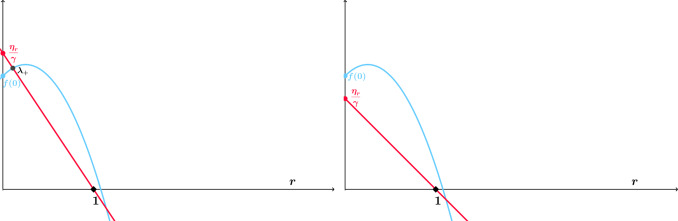
\includegraphics[width=0.7\textwidth]{1-s2.0-S1007570424005975-gr3.jpg}
		\caption{\(f\) and \(\lambda_+\)}
	\end{figure}
	
	\item Case 5:  \(s \neq 0 \ , \ r = 0 \ , \ p = 0 \)
	
	Here, we have the equilibrium $E_3(1,1-\frac{\alpha}{\eta_s},0,0)$ which exists if $\alpha<\eta_s$.
	
	\newpage
	\item Case 6:  \(s \neq 0 \ , \ r = 0 \ , \ p \neq 0 \)
	
	In this scenario, $s=\lambda_-$ and $p = f(\lambda_-)$, where $0 < \lambda_- < 1$ is the unique solution of this equation:
	\begin{equation}
		f(s) = \frac{\eta_s- \alpha}{\gamma} - \frac{\eta_s}{\gamma}s
	\end{equation}
	which exists for $f(0) < \frac{\eta_s- \alpha}{\gamma}$.
	
	\begin{figure}[h!]
		\centering
		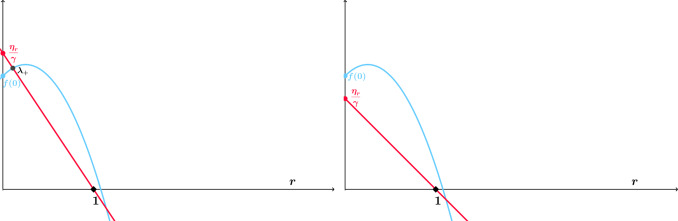
\includegraphics[width=0.7\textwidth]{1-s2.0-S1007570424005975-gr3.jpg}
		\caption{\(f\) and \(\lambda_-\)}
	\end{figure}

	

	\item Case 7:   \(s \neq 0 \ , \ r \neq 0 \ , \ p \neq 0 \)
	In this case, we obtain $n_* = s + r = 1 - \frac{\alpha + \beta}{\eta_s - \eta_r}$.
	
	This value of $n_*$ is positive under the condition that $\alpha + \beta + \eta_r < \eta_s$, hence, we have $p_* = f(n_*)$. Furthermore, the equations for $s_*$ and $r_*$ are given by:
	$$s_* = \frac{n_*}{\beta}\left( \gamma f(n_*) - \eta_r \frac{\alpha + \beta}{\eta_s - \eta_r} \right)$$
	$$r_* = \frac{n_*}{\beta}\left( \eta_s \frac{\alpha + \beta}{\eta_s - \eta_r} - \alpha - \gamma f(n_*) \right)$$
	and these values are positive under the condition
	$$\eta_r \frac{\alpha + \beta}{\eta_s - \eta_r} < \gamma f(n_*) < \frac{\alpha \eta_r + \beta \eta_s}{\eta_s - \eta_r}.$$
	
\end{itemize}


	
	
	
	\newpage
	\section{Stability Analysis} Local stability is determined by the signs of the eigenvalues of the Jacobian matrix obtained by linearizing our system around the steady state. This is given at any point $J(a,s,r,p)$ by
$$\begin{pmatrix}
	-\mu & 0 & 0 & 0 \\
	-\alpha s & \eta_s (1-n) - \eta_s s - \alpha a - \beta \frac{r^2}{n^2} - \gamma p & -\eta_s s - \beta \frac{s^2}{n^2} & -\gamma s \\
	0 & -\eta_r r + \beta \frac{r^2}{n^2} & \eta_r (1-n) - \eta_r r + \beta \frac{s^2}{n^2} - \gamma p & -\gamma r \\
	0 & \phi(n) (f(n)-p) + \dot{f}(n) p \phi(n) & p \dot{\phi}(n) (f(n)-p) + \dot{f}(n) p \phi(n) & \phi(n) (f(n)-2p)
\end{pmatrix}.$$


We denote Locally Asymptotically Stable as LAS. Moreover, we use the notations below
$$C_{+} = \eta_{s}\left(1 - \lambda_{+}\right) - \alpha - \beta$$
$$ C_{-} = \eta_{r}\left(1 - \lambda_{-}\right) + \beta$$
$$C_* = -\frac{\left(\eta_s s_* + \eta_r r_*\right) \beta s_* r_* \left(\eta_s - \eta_r\right)}{f(n_*)\phi(n_*) (n_*)^2 \left(\eta_s s_* + \eta_r r_* + f(n_*)\phi(n_*)\right)} - \frac{\eta_s s_* - \eta_r r_*}{\eta_*} .$$

\begin{theo}

\ 	\begin{enumerate}
		\item The equilibrium \( E_2 \ (1, 0, 1, 0) \) is unstable.
		\item The equilibrium \( E_3 \left(1, 1 - \frac{\alpha}{\eta_s}, 0, 0\right) \) is unstable.
		\item The equilibrium \( E_+ \ (1, 0, \lambda_+, f(\lambda_+) ) \) is LAS iff $\gamma f(\lambda_+)> C_+$ and $\gamma \dot f(\lambda_+)> \eta_r$.
		\item The equilibrium 
		\( E_- \ (1, \lambda_-, 0, f(\lambda_-)) \) is LAS iff $\gamma f(\lambda_-)>C_- $ and 
		$\gamma \dot f(\lambda_-)>\eta_s$.
		\item The equilibrium \( E_* \ (1, s_*, r_*, f(n_*) ) \) is LAS iff $\gamma \dot f(n_*)>C_*$.
	\end{enumerate}
\end{theo}
\begin{proof}
\	\begin{enumerate}
		\item Equilibrium \(E_{2}(1,0,1,0)\):  
		The Jacobian matrix of the equilibrium \(E_{2}\) is given by  
		\[
		J(E_{2}) = \begin{pmatrix} 
			-\mu & 0 & 0 & 0 \\ 
			0 & -a-\beta & 0 & 0 \\ 
			0 & -\eta_{r} + \beta & -\eta_{r} & -\gamma \\ 
			0 & 0 & 0 & \phi(1)f(1) 
		\end{pmatrix}.
		\]
		Given that \(\phi(1)f(1)>0\), it follows that \(E_{2}\) is an unstable point.
		
		\item Equilibrium \(E_{3}\left(1,1-\dfrac{\alpha}{\eta_{s}},0,0\right)\):  
		The Jacobian matrix corresponding to the equilibrium point \(E_{3}\) is represented as  
		\[
		J(E_{3}) = \begin{pmatrix} 
			-\mu & 0 & 0 & 0 \\ 
			\dfrac{\alpha^{2}}{\eta_{s}} - \alpha & \alpha - \eta_{s} & \alpha - \eta_{s} - \beta & -\gamma + \dfrac{\gamma\alpha}{\eta_{s}} \\ 
			0 & 0 & \dfrac{\eta_{r}\alpha}{\eta_{s}} + \beta & 0 \\ 
			0 & 0 & 0 & \phi\left(1-\dfrac{\alpha}{\eta_{s}}\right)f\left(1-\dfrac{\alpha}{\eta_{s}}\right) 
		\end{pmatrix}.
		\]
		Since \(\phi\left(1-\dfrac{\alpha}{\eta_{s}}\right)f\left(1-\dfrac{\alpha}{\eta_{s}}\right)>0\), this indicates that the equilibrium \(E_{3}\) is unstable.
		\item Equilibrium \(E_{+}(1,0,\lambda_{+},f(\lambda_{+}))\): The Jacobian matrix associated with the equilibrium point \(E_{+}\) is expressed as
		$$
		J(E_{+}) = \begin{pmatrix}
			-\mu & 0 & 0 & 0 \\ 
			0 & \eta_{s}(1-\lambda_{+})-\alpha-\beta-\gamma f(\lambda_{+}) & 0 & 0 \\ 
			0 & -\eta_{r}\lambda_{+} + \beta & -\eta_{r}\lambda_{+} & -\gamma\lambda_{+} \\ 
			0 & f(\lambda_{+})f(\lambda_{+})\phi(\lambda_{+}) & f(\lambda_{+})f(\lambda_{+})\phi(\lambda_{+}) & -f(\lambda_{+})\phi(\lambda_{+})
		\end{pmatrix}.
		$$
		
		The eigenvalues of the Jacobian matrix \(J(E_{+})\) are expressed as:
		\[
		\lambda_{1} = -\mu,
		\]
		\[
		\lambda_{2} = \eta_{s}(1-\lambda_{+})-\alpha-\beta-\gamma f(\lambda_{+}).
		\]
		
		The remaining eigenvalues, \(\lambda_{3}\) and \(\lambda_{4}\), are given from the matrix \(B\):
		\[
		B = \begin{pmatrix}
			-\eta_{r}\lambda_{+} & -\gamma\lambda_{+} \\ 
			\dot{f}(\lambda_{+})f(\lambda_{+})\phi(\lambda_{+}) & -f(\lambda_{+})\phi(\lambda_{+})
		\end{pmatrix}.
		\]
		
		We have
		\[
		\operatorname{tr}(B) = -\eta_{r}\lambda_{+} - f(\lambda_{+})\phi(\lambda_{+}) < 0
		\]
		and
		\[
		\det(B) = \lambda_{+}f(\lambda_{+})\phi(\lambda_{+})(\eta_{r} + \gamma f(\lambda_{+})).
		\]
		
		Consequently, the eigenvalues have a negative real part if and only if
		\[
		(\eta_{s}-\eta_{r})(1-\lambda_{+}) < \alpha + \beta, \quad f(\lambda_{+}) > -\dfrac{\eta_{r}}{\gamma}.
		\] 
		
		
		\item Equilibrium \(E_{-}(1,\lambda_{-},0,f(\lambda_{-}))\): The Jacobian matrix corresponding to the equilibrium point \(E_{-}\) is
		\[
		J(E_{-}) = \begin{pmatrix}
			-\mu & 0 & 0 & 0 \\ 
			-\alpha\lambda_{-} & -\eta_{s}\lambda_{-} & -\eta_{s}\lambda_{-} - \beta & -\gamma\lambda_{-} \\ 
			0 & 0 & \eta_{r}(1-\lambda_{-}) + \beta - \gamma f(\lambda_{-}) & 0 \\ 
			0 & f(\lambda_{-})f(\lambda_{-})\phi(\lambda_{-}) & f(\lambda_{-})f(\lambda_{-})\phi(\lambda_{-}) & -f(\lambda_{-})\phi(\lambda_{-})
		\end{pmatrix}.
		\]
		
		The eigenvalues of the Jacobian matrix \(J(E_{-})\) are determined as follows:
		\[
		\lambda_{1} = -\mu,
		\]
		\[
		\lambda_{2} = \eta_{s}(1-\lambda_{-}) + \beta - \gamma f(\lambda_{-}).
		\]
		
		For the additional eigenvalues, \(\lambda_{3}\) and \(\lambda_{4}\), they are calculated from matrix \(C\):
		\[
		C = \begin{pmatrix}
			-\eta_{s}\lambda_{-} & -\gamma\lambda_{-} \\ 
			\dot{f}(\lambda_{-})f(\lambda_{-})\phi(\lambda_{-}) & -f(\lambda_{-})\phi(\lambda_{-})
		\end{pmatrix}.
	\]

Since
\[
\operatorname{tr}(C) = -\eta_{s}\lambda_{-} - f(\lambda_{-})\phi(\lambda_{-}) < 0
\]
and
\[
\det(C) = \lambda_{-}f(\lambda_{-})\phi(\lambda_{-})(\eta_{s} + \gamma f(\lambda_{-})),
\]

then, the eigenvalues have a negative real part if and only if
\[
(\eta_{s} - \eta_{r})(1 - \lambda_{-}) > a + \beta, \quad f(\lambda_{-}) > \frac{\eta_{s}}{\gamma}.
\]
		
		\item Equilibrium \(E_{*}(1,s_{*},r_{*},f(n_{*}))\): We investigate below the local stability of \(E_{*}\). The Jacobian matrix of our system at \(E_{*}\) takes the form 
		\[
		J(E_{*}) = \begin{pmatrix}
			-\mu & 0 & 0 & 0 \\ 
			-\alpha s_{*} & -\eta_{s}s_{*} + \beta\dfrac{s_{*}r_{*}}{n_{*}^{2}} & -\eta_{s}s_{*} - \beta\dfrac{s_{*}}{n_{*}} + \beta\dfrac{s_{*}r_{*}}{n_{*}^{2}} & -\gamma s_{*} \\ 
			0 & -\eta_{r}r_{*} + \beta\dfrac{r_{*}}{n_{*}} - \beta\dfrac{s_{*}r_{*}}{n_{*}^{2}} & -\eta_{r}r_{*} - \beta\dfrac{s_{*}r_{*}}{n_{*}^{2}} & -\gamma r_{*} \\ 
			0 & f(n_{*})f(n_{*})\phi(n_{*}) & f(n_{*})f(n_{*})\phi(n_{*}) & -f(n_{*})\phi(n_{*})
		\end{pmatrix}.
		\]
		
		The characteristic polynomial of \(J(E_{*})\) is given by
		$$P(\lambda) = -(\lambda + \mu)\left(
		\lambda^{3} - \operatorname{tr}(D)\lambda^{2} 
		- \frac{1}{2}\left[\operatorname{tr}(D^{2}) - (\operatorname{tr}(D))^{2}\right]\lambda 
		- \det(D)
		\right),$$
		where \(D\) is the following matrix:
		\[
		D = \begin{pmatrix}
			-\eta_{s}s_{*} + \beta\dfrac{s_{*}r_{*}}{n_{*}^{2}} & 
			-\eta_{s}s_{*} - \beta\dfrac{s_{*}}{n_{*}} + \beta\dfrac{s_{*}r_{*}}{n_{*}^{2}} & 
			-\gamma s_{*} \\[2ex]
			-\eta_{r}r_{*} + \beta\dfrac{r_{*}}{n_{*}} - \beta\dfrac{s_{*}r_{*}}{n_{*}^{2}} & 
			-\eta_{r}r_{*} - \beta\dfrac{s_{*}r_{*}}{n_{*}^{2}} & 
			-\gamma r_{*} \\[2ex]
			f(n_{*})f(n_{*})\phi(n_{*}) & 
			f(n_{*})f(n_{*})\phi(n_{*}) & 
			-f(n_{*})\phi(n_{*})
		\end{pmatrix}.
		\]
		Therefore, the primary eigenvalue is \(\lambda_{1} = -\mu\), while the remaining eigenvalues are solutions to the cubic equation
		\begin{equation}
			\lambda^{3} + a_{2}\lambda^{2} + a_{1}\lambda + a_{0} = 0, \tag{10}
		\end{equation}
		with coefficients defined as follows:
		\[
		a_{2} = -\operatorname{tr}(D), \quad 
		a_{1} = -\frac{1}{2}\left[\operatorname{tr}(D^{2}) - (\operatorname{tr}(D))^{2}\right], \quad 
		a_{0} = -\det(D).
		\]
		
		Per the Routh-Hurwitz criterion for third-order polynomials, all solutions of the equation are situated in the left half of the complex plane if and only if \(a_{2} > 0\), \(a_{0} > 0\), and \(a_{2}a_{1} > a_{0}\). Detailed computations yield
		\begin{align*}
			a_{0} &= f(n_{*})\phi(n_{*})\beta\frac{s_{*}r_{*}}{n_{*}}(\eta_{s} - \eta_{r}) > 0 \\
			a_{2} &= \eta_{s}s_{*} + \eta_{r}r_{*} + f(n_{*})\phi(n_{*}) > 0,
		\end{align*}
		and
		\begin{align*}
			a_{1}a_{2} - a_{0} 
			&= f(n_{*})\phi(n_{*})(\eta_{s}s_{*} + \eta_{r}r_{*})(\eta_{s}s_{*} + \eta_{r}r_{*} + f(n_{*})\phi(n_{*})) \\
			&\quad + (\eta_{s}s_{*} + \eta_{r}r_{*})\beta\frac{s_{*}r_{*}}{n_{*}}(\eta_{s} - \eta_{r}) > 0 \quad \square
		\end{align*}
		
		
		
		
		
		
		
		
	\end{enumerate}
\end{proof}
\begin{prp}
	The equilibrium \( E_0(1,0,0,0) \) is unstable.
\end{prp}
\begin{proof}
	Assume, by way of contradiction, that for an initial condition \((a(0),s(0),r(0),p(0))\) near \(E_0\), it holds that
	\[
	\lim_{t \to +\infty} s(t) = \lim_{t \to +\infty} r(t) = \lim_{t \to +\infty} p(t) = 0.
	\]
	Since \(f\) and \(\phi\) are continuous functions, we have
	\[
	\lim_{t \to +\infty} f(u(t)) = f(0), \quad \lim_{t \to +\infty} \phi(u(t)) = \phi(0).
	\]
	Thus, for any \(\epsilon > 0\), there exists \(\tilde{t} > 0\) such that for all \(t \geq \tilde{t}\), the following conditions are satisfied:
	\[
	f(u(t)) \geq f(0) - \epsilon \quad \text{and} \quad \phi(u(t)) \geq \phi(0) - \epsilon.
	\]
	For all \(t \geq \tilde{t}\), the function \(p(t)\) satisfies
	\begin{align*}
		p(t) &= p\phi(n)(f(n) - p) \\
		&\geq p\phi(n)(f(0) - \epsilon - p) \\
		&\geq p(\phi(0) - \epsilon)(f(0) - \epsilon) \left( 1 - \frac{p}{f(0) - \epsilon} \right).
	\end{align*}
	This yields
	\[
	\liminf_{t \to +\infty} p(t) \geq f(0) - \epsilon.
	\]
	As \(\epsilon > 0\) was chosen arbitrarily, we conclude that \(\liminf_{t \to +\infty} p(t) \geq f(0)\), which contradicts our initial assumption.
\end{proof}
\begin{theo}
	The equilibrium $E_1$ is LAS if $\alpha>\eta_s$ and $\gamma f(0) > \eta_r $.
\end{theo}
\begin{proof}
	First, \(\lim_{t \to +\infty} a(t) = 1\). Substituting this value into the second equation of our system we obtain the asymptotically equivalent system given by
	\begin{equation}
	\begin{cases}
		\dot{s}(t) &= \eta_s (1 - n)s - as - \beta \frac{sr}{n} - ysp, \\
		\dot{r}(t) &= \eta_r (1 - n)r + \beta \frac{sr}{n} - yrp, \\
		\dot{p}(t) &= \phi(n)p(f(n) - p), \\
		n &= s + r.
	\end{cases}
	\end{equation}
	
	The first equation gives
	\begin{align*}
		\dot{s}(t) &= \eta_s (1 - n)s - as - \beta \frac{sr}{n} - ysp \\
		&\leq (\eta_s - a)s
	\end{align*}
	which implies that \(\lim_{t \to +\infty} s(t) = 0\). Substituting this value into the second equation we obtain the asymptotically equivalent system as follows
	
	\begin{equation}
	\begin{cases}
		\dot{r}(t) &= \eta_r (1 - r)r - yrp, \\
		\dot{p}(t) &= \phi(r)p(f(r) - p).
	\end{cases}
	\end{equation}
	
	The Jacobian matrix associated with the point \((0, f(0))\) of this planar system is given by
	\[
	\begin{pmatrix}
		\eta_r - yf(0) & 0 \\
		f(0)f(0)\phi(0) & -f(0)\phi(0)
	\end{pmatrix}
	\]
	which completes our proof. \qedhere
\end{proof}

\begin{table}[ht]
	\centering
	\caption{Conditions for the stability of equilibria.}
	\label{tab:stability}
	\begin{tabular}{l|l|l}
		\hline
		\textbf{Equilibrium} & \textbf{Biological existence} & \textbf{Stability} \\
		\hline
		\hline
		\( E_0 \ (1, 0, 0, 0) \) & Always exists & Always unstable \\ 
		\( E_1 \ (1, 0, 0, f(0)) \) & Always exists & \(\alpha > \eta_s\) and \(\gamma f(0) > \eta_r\) \\
		\( E_2 \ (1, 0, 1, 0) \) & Always exists & Always unstable \\
		\( E_3 \left(1, 1 - \frac{\alpha}{\eta_s}, 0, 0\right) \) & \(\eta_s > \alpha\) & Always unstable \\
		\( E_+ \ (1, 0, \lambda_+, f(\lambda_+) ) \) & \(\eta_r > \gamma f(0)\) & \(\gamma f(\lambda_+) > C_+\) and \(\gamma f(\lambda_+) > \eta_r\) \\
		\( E_- \ (1, \lambda_-, 0, f(\lambda_-)) \) & \(\eta_s - \alpha > \gamma f(0)\) & \(\gamma f(\lambda_-) > C_-\) and \(\gamma f(\lambda_-) > \eta_s\) \\
		\( E_* \ (1, s_*, r_*, f(n_*) ) \) & 
		\(\begin{cases}
			\eta_r \frac{\alpha + \beta}{\eta_s - \eta_r} < \gamma f(n_*) < \frac{\eta_r \alpha + \eta_s \beta}{\eta_s - \eta_r} \\
			\text{and} \\
			\eta_s > \eta_r + \alpha + \beta
		\end{cases}\) & 
		\(\gamma f(n_*) > C_*\) \\
		\hline
		\hline
	\end{tabular}
\end{table}
	
	
	\newpage
	\section{Numerical Computation and Results} Our mathematical model sheds light on the intricate dynamics of antibiotic resistance and provides a theoretical framework for devising effective intervention strategies. By identifying stable equilibria and delineating distinct biological scenarios, our model offers valuable insights into the interplay between antibiotic-resistant bacteria, the immune response, and antibiotic treatment. Our model is characterized by a system of four differential equations.

\begin{table}[ht]
	\centering
	\caption{The selection of parameters}
	\label{tab:parameters}
	\begin{tabular}{cccc}
		\hline
		\textbf{$E_1$} & \textbf{$E_+$} & \textbf{$E_-$} & \textbf{$E_*$} \\ 
		\hline
		$\alpha = 1$ 	& $\alpha = 0.2$ 	& $\alpha = 1$ 	& $\alpha = 0.1$ \\
		$\beta = 0.1$ 	& $\beta = 0.3$ 		& $\beta = 0.1$ & $\beta = 1.7$ \\
		$\gamma = 1$ 	& $\gamma = 1$ 		& $\gamma = 1$ 	& $\gamma = 1$ \\
		$\eta_s = 1$ 	& $\eta_s = 2$ 		& $\eta_s = 4$ 	& $\eta_s = 3$ \\
		$\eta_r = 0.3$ 	& $\eta_r = 2.5$ 	& $\eta_r = 1$ 	& $\eta_r = 0.5$ \\
		$\mu = 3$ 		& $\mu = 3$ 		& $\mu = 3$ 	& $\mu = 3$ \\
		\hline
	\end{tabular}
\end{table}
0.1, 1.4, 1, 3, 0.5, 3

Initially, we establish the presence of a positively invariant set, indicating a natural constraint on growth due to limited resources, as expressed in the logistic growth term.

\begin{figure}
	\centering
	\caption{Equilibria of $E_1$}
	\label{fig:e1}
	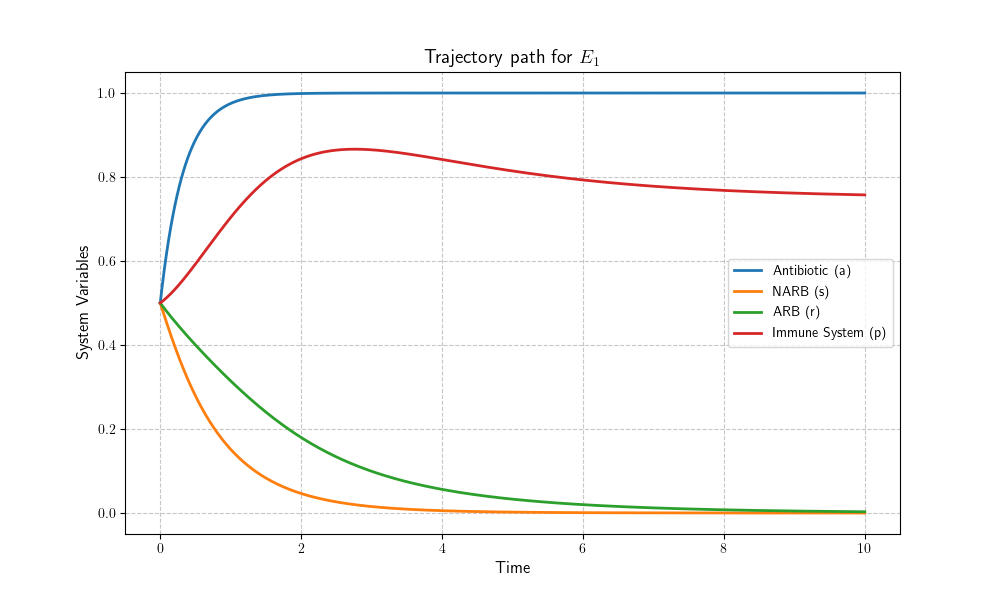
\includegraphics[width = 0.7\textwidth]{E_1.png}
\end{figure}


Additionally, the qualitative investigation reveals the presence of four stable equilibria. The stability of the equilibrium point $E_1 \left(1, 0, 0, f(0)\right)$ is clarified through specific limit calculations, which provide insights into the behavior of the system under certain conditions. This equilibrium represents a state where the infection has been cleared from the system. From a biological perspective, the stability of $E_1$ implies that the system can reach this infection-free state when key parameters align favorably. Specifically, for $E_1$ to be stable, two crucial conditions must be met: First, the antibiotic must be administered at a sufficiently high rate compared to the reproduction rate of non-resistant bacteria. This ensures that the population of non-resistant bacteria is suppressed effectively. Second, the immune response must be strong enough to outcompete and eliminate resistant bacteria. When both of these conditions are satisfied, the system can overcome the infection, leading to the eventual disappearance of the bacterial population.


\begin{figure}
    \centering
    \caption{Equilibria of $E_+$ and $E_-$}
    \begin{subfigure}{0.49\textwidth}\label{fig:epos}
        \centering
        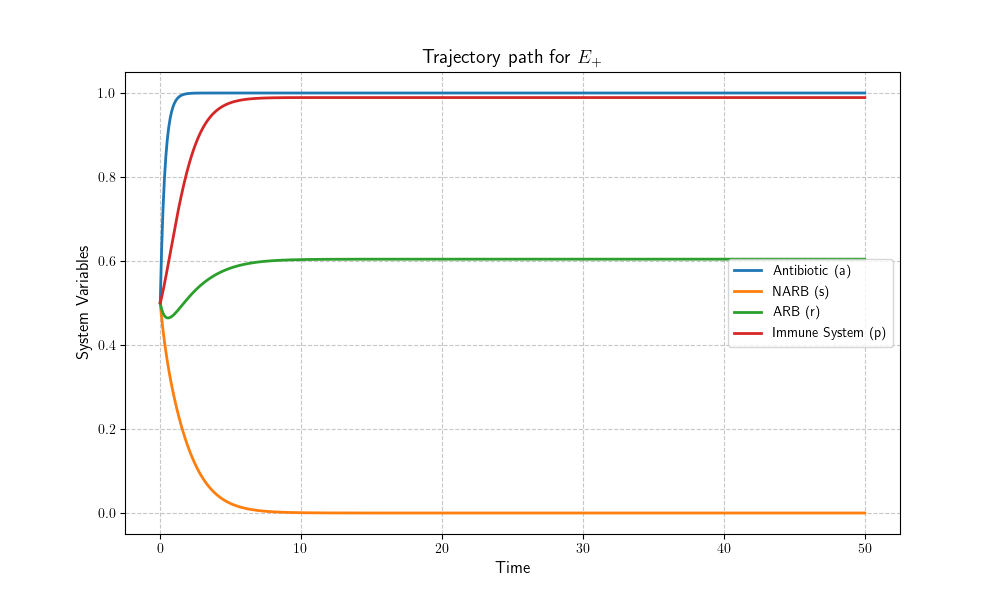
\includegraphics[width =\textwidth]{E_pos.png}
    \end{subfigure}
    \begin{subfigure}{0.49\textwidth}\label{fig:eneg}
        \centering
        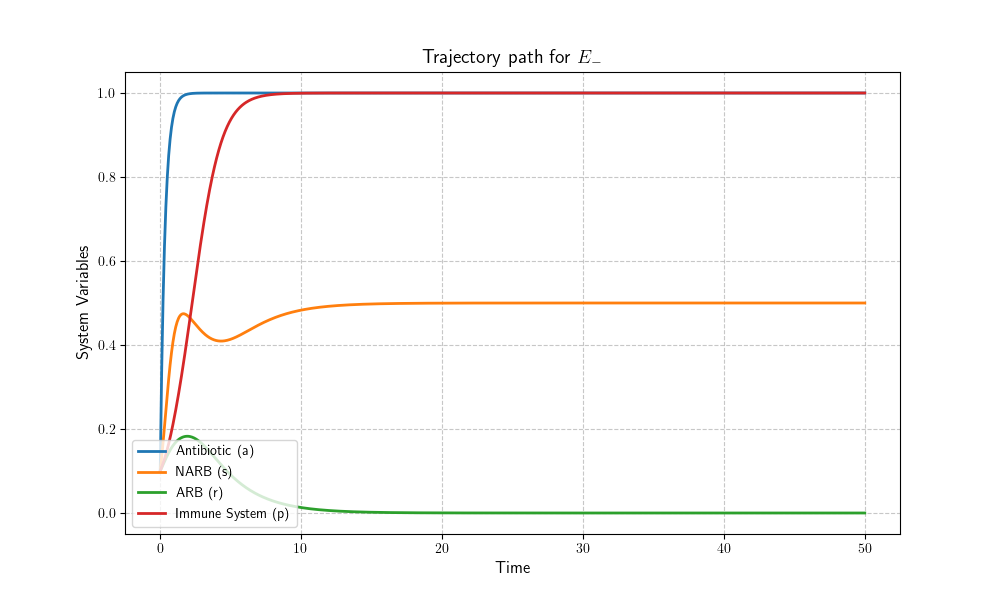
\includegraphics[width = \textwidth]{E_neg.png}
    \end{subfigure}
\end{figure}

The stability analysis of the equilibria $E_+$ and $E_-$ is provided through the Lyapunov theory, which provides a rigorous mathematical framework for assessing the stability of these points in the system. In terms of biology, $E_+$ describes a situation where the infection is sustained entirely by resistant bacteria. At this point, the antibiotic is effective in eliminating non-resistant bacteria, which means that the non-resistant strain is unable to survive in the presence of the treatment. However, the resistant bacteria continue to propagate, suggesting that the antibiotic is not effective against them. This scenario highlights the challenge posed by antibiotic resistance: even with a strong treatment, the infection persists due to the presence of bacteria that can withstand the antibiotic. The stability of $E_+$ implies that under certain conditions—specifically, when the resistant bacteria have a survival advantage—the system will remain in this state unless external interventions are made to counteract the resistance.


In contrast, the equilibrium $E_-$ represents a different biological outcome. Here, the infection is driven entirely by non-resistant bacteria, with the resistant strain being eliminated. This situation arises when the antibiotic dosage is insufficient to suppress the non-resistant bacteria fully, allowing them to continue propagating. However, the resistant bacteria are outcompeted by the immune system because their reproduction rate is lower compared to the strength of the immune response. In this scenario, while the non- resistant bacteria remain problematic, the resistant bacteria do not pose a threat, indicating that the infection can still be controlled if the immune response is sufficiently strong. The stability of $E_*$ suggests that under certain conditions, the system can settle into a state where non-resistant bacteria dominate, but the resistant bacteria are eradicated.

\begin{figure}\label{fig:estar}
    \centering
    \caption{Equilibria of $E_*$}
    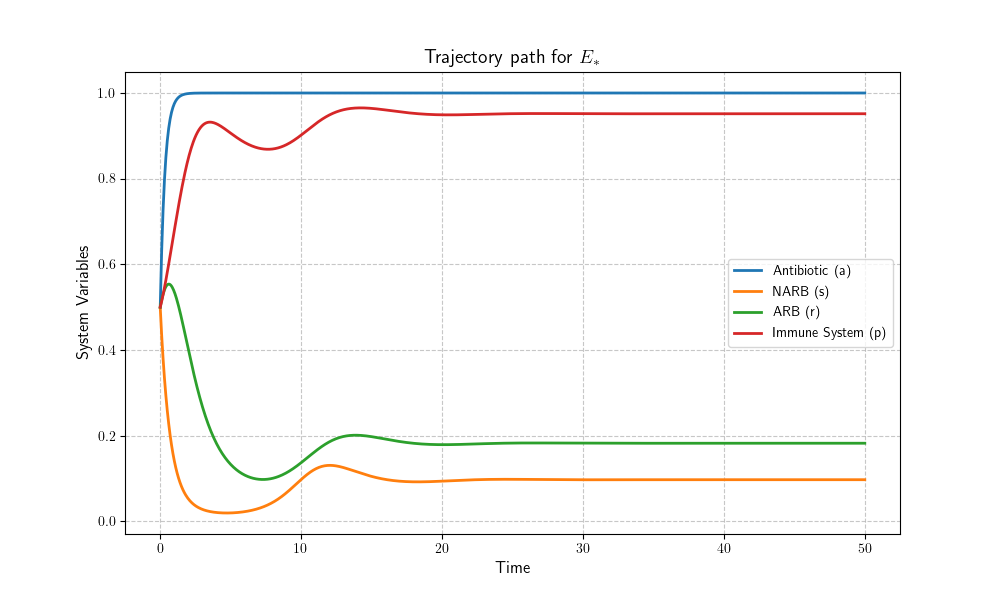
\includegraphics[width = 0.7\textwidth]{E_star.png}
\end{figure}


Ultimately, the stability of $E_* \left(1, s_* , r_* , f (n_*)\right)$ is established through the combined application of the Lyapunov theory and the Routh criteria theorem. In biological terms, the stability of $E_*$ indicates that neither the antibiotic nor the immune response alone can eradicate the infection instigated by both non-resistant and resistant bacteria. In this scenario, a good approach involves incrementally raising the antibiotic dosage within reasonable limits. Indeed, according to the World Health Organization (WHO), widespread antibiotic usage fosters the evolution of resistance in bacteria, prompting them to develop mechanisms to counteract the antibiotic's effects. So ideally, combining the antibiotic with an antivirulence treatment would be optimal. In fact, the latest studies show that employing anti-virulence therapeutic strategies against bacterial infections emerges as the most effective biological approach for eradicating the bacterial infection. Microorganisms possess diverse resistance mechanisms against various classes of antibiotics, underscoring the imperative to uncover novel antimicrobial compounds for combating bacterial infections. A compelling and innovative approach to neutralizing pathogens involves antivirulence therapy, which entails inhibiting bacterial virulence factors or pathogenicity. Consequently, integrating these novel pathoblockers into treatment regimens could diminish the necessity for broad-spectrum antimicrobial administration and curb the prevalence of resistant strains. Introducing antivirulence treatment into our future study would be highly intriguing from a modeling perspective.


Another aspect to consider concerning the equilibrium point $E_*$ is whether the density of resistant bacteria surpasses that of non-resistant bacteria. This holds significant biological importance in combating the infection. In fact, if the condition
\[
2\gamma f\left(1 - \frac{\alpha + \beta}{\eta_S - \eta_T}\right) + \alpha \geq (\eta_S + \eta_T)\frac{\alpha + \beta}{\eta_S - \eta_T} 
\]

is satisfied, then $s_* \ge r_*$.

In future research, exploring the spatiotemporal dynamics of bacterial infection spreading in tissues would be particularly intriguing. Notably, research has demonstrated variations in infection spread across different tissues, organs, and the bloodstream.

	
	
	\newpage
	\addcontentsline{toc}{section}{References}
	\nocite{*}
	\printbibliography
	
	
\end{document}
 